\chapter{基于信息熵的数据商品在线拍卖的研究}

\section{研究动机}
随着近些年人们产生的数据量的巨量增长,关于数据交易的市场雏形可见,并可期成为一个巨大规模的市场。然而,现有的关于传统商品的交易和定价策略是不适用于数据商品的,因为这些交易和定价策略均不能最大化交易双方的总剩余,从而打击交易的积极性和信心。而数据,这一新商品,目前其交易场景多为线上。从而,交易双方的信心和积极性是促成数据交易的关键因素。目前,在这个数据交易市场上,数据买家远多于卖家,使得这个市场近似于一个寡头竞争市场。基于以上两点,我们发现拍卖可能会是一个很好的数据商品定价和交易的机制。一是因为其能最大化交易双方的总剩余,二是因为拍卖机制中本来就有为这种寡头竞争市场专门设计的规则。但这不意味着我们可以直接把为传统商品设计的拍卖机制直接应用到数据商品上,因为数据商品和传统商品有很大的区别。相比于传统商品,数据商品具有唯一性和不确定均衡价格。

在众多关于拍卖的研究文献中\cite{Vickrey1961Counterspeculation,Milgrom1989Auctions,Milgrom1982A,Riley1981Optimal},拍卖物的价值$v$被认为是服从一个均匀分布,即$v\sim U[v_l,v_h]$,其中$v_l$是估价的下限,$v_h$是估价的上限。但是这些文献均没有给出如何估计上下限的指导方法,而估值上下限却是实施拍卖机制的基础。相比于传统商品,数据商品更无形,更加抽象,因此更难以被普通消费者估计它们的价值。尽管现在已经有一些关于数据商品的评价指标,比如数据集大小,数据集生成时间等,但这仍是远远不够的。我们需要找一个更合适的指标来评估数据集,从而指导拍卖参与者对数据商品的估价。目前,Li等人\cite{li2017first}提出了数据信息熵这一新的指标,用来测定给定数据集的信息量和清晰地描述数据集内的信息分布,在他们文中还提出了一系列基于该指标定价的好处。数据信息熵可能是一个非常合适的帮助数据商品估价的指标,我们期望先用数据信息熵测定给定数据商品的信息量,然后基于它给出该商品的估值上下限,从而实施拍卖机制。

\section{影响在线拍卖的重要因素}
文献\cite{Pinker2003Managing}提出了一些影响在线拍卖的重要因素,但是没有真实拍卖交易数据的支持。因此,我们收集了2012年12月到2013年eBay Live Auction的一些交易记录,希望以此佐证文献\cite{Pinker2003Managing}提出的这些影响因素。这些数据集包含了Cartier手表,Palm Pilot M515掌上智能机,Xbox游戏终端以及Swarovski珍珠项链在这段时期的相关拍卖信息。具体来说,它包含了相关的九个变量,即拍卖入场时间,拍卖持续时长,成交价等。在这个数据集中,总共有三种类型的拍卖,分别是时长为3天的拍卖,时长为5天的拍卖和时长为7天的拍卖。为了能挖掘拍卖价格,入场时间以及拍卖持续时长的关系,我们将该数据集中部分记录进行了可视化,如图\ref{fig:number of bidders distribution histogram}。这些可视化帮助我们更加清晰地认知这些因素是如何影响拍卖的。以下是我们在设计数据商品在线拍卖模型时最关心的三个因素。

\subsection{拍卖机制}

第一价格拍卖、第二价格拍卖、英式增价拍卖、荷兰式减价拍卖是目前用的最多也是被研究的最多的四种拍卖机制。其中,英式增价拍卖在在线网络拍卖中是用得最多的,因为它是顾客最熟悉、接触最多的拍卖机制。目前,最大的在线拍卖网站,eBay Live Auction 采用的正是英式拍卖。eBay Live Auction已成功吸引了数以百万计的人参与他们的在线拍卖,这从侧面佐证了英式增价拍卖的可用性。

然而, Milgrom等人\cite{Milgrom1989Auctions}提出英式拍卖机制容易受到不同欺诈行为的影响。Pinker等人\cite{Pinker2001Using,Pinker2003Managing}认为一个好的拍卖机制必须居然三个特指:1)对不同顾客行为鲁棒的;2)分配是要高效的;3)要能有效应对欺诈行为的。设计一个最优拍卖仅仅是存在于理论中的,因为最优拍卖机制中的许多假设在现实中是难以满足的。另外,理论上的最优拍卖机制在市场中是难以实现的。Myerson\cite{Myerson1981Optimal}在上述四个拍卖机制下提出了收益均衡定理。Lucking-Reiley\cite{Lucking1999Using}通过对邮票的在线拍卖的实验,比较了英式拍卖和第二价格拍卖的收入产生。他们的目标是去验证Myerson的收益等价定理在英式拍卖和第二价格拍卖下是否成立。他们发现,这二者的最终收益的差别是非常小的,因此我们也认为在线英式拍卖的理论经验是可靠的。

大量关于在线拍卖的研究是集中在前向拍卖 (forward auction), 即是一个卖家向多个买家拍卖物品。以上提到的四个拍卖机制均是前向拍卖。然而,还是存在另外一大类拍卖,反向拍卖 (reverse auction),即一个买家需要买一件物品,多个卖家以竞争的方式提供该物品,这个场景多出现在政府项目招标中。然而,对于数据的在线拍卖,是不太适合使用反向拍卖作为拍卖机制的,因为目前市场上并没有足够多的数据提供商去满足众多数据买家的需求。

\subsection{竞拍时长与参与人数}

竞拍时长在在线拍卖中有着很大的作用。相比于传统的只持续数十分钟或数个小时的传统公开拍卖,在线拍卖往往会持续数天或数周。因为在线拍卖不会要求竞拍人到场,他们能在任何地点任何时间参与拍卖\cite{Pinker2003Managing}。因此,持续时间很长的在线拍卖是可行的。传统拍卖往往会以一个固定的竞拍人数开始拍卖,而相应的关于期望收益和最优保留价的分析都是基于这固定的竞拍人数的。但是,同样的分析方法就不适用于在线拍卖。因为,在网络上,在线拍卖的人数是不固定的,而在线拍卖的竞拍人数往往是由竞拍时长决定的。

\begin{figure}
   \centering
   \subfigure[持续时长为3天的拍卖]{
     \label{fig:3-day auction} %% label for first subfigure
     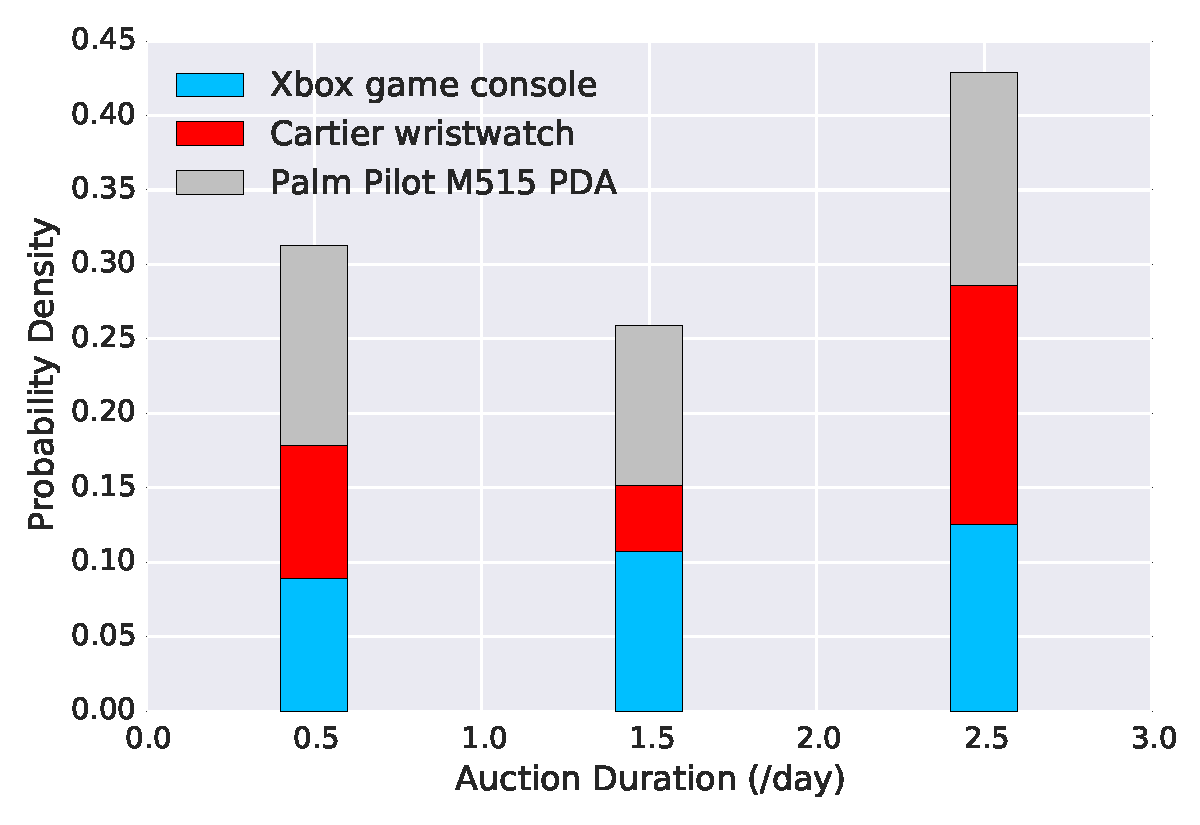
\includegraphics[width=0.55\textwidth]{chapter4/3_days_hist}}
   \subfigure[持续时长为5天的拍卖]{
     \label{fig:5-day auction} %% label for second subfigure
     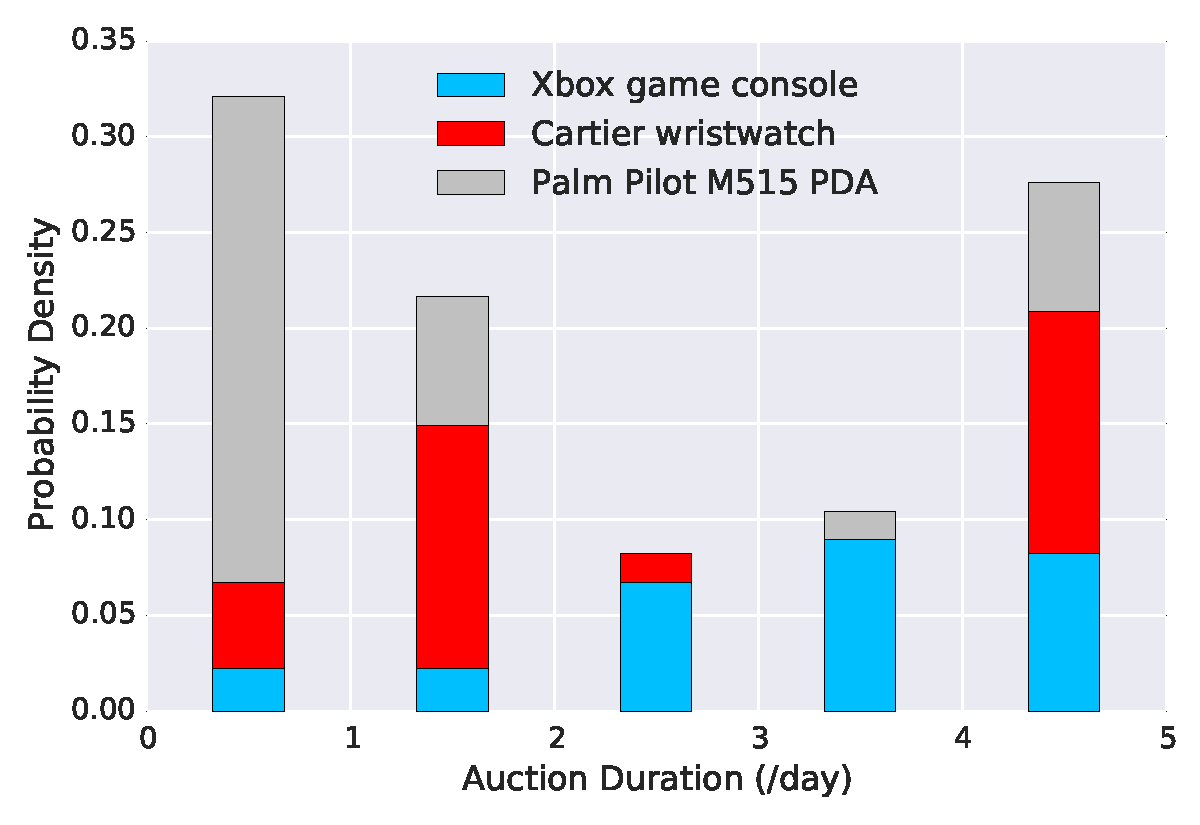
\includegraphics[width=0.55\textwidth]{chapter4/5_days_hist}}
   \subfigure[持续时长为7天的拍卖]{
     \label{fig:7-day auction} %% label for second subfigure
     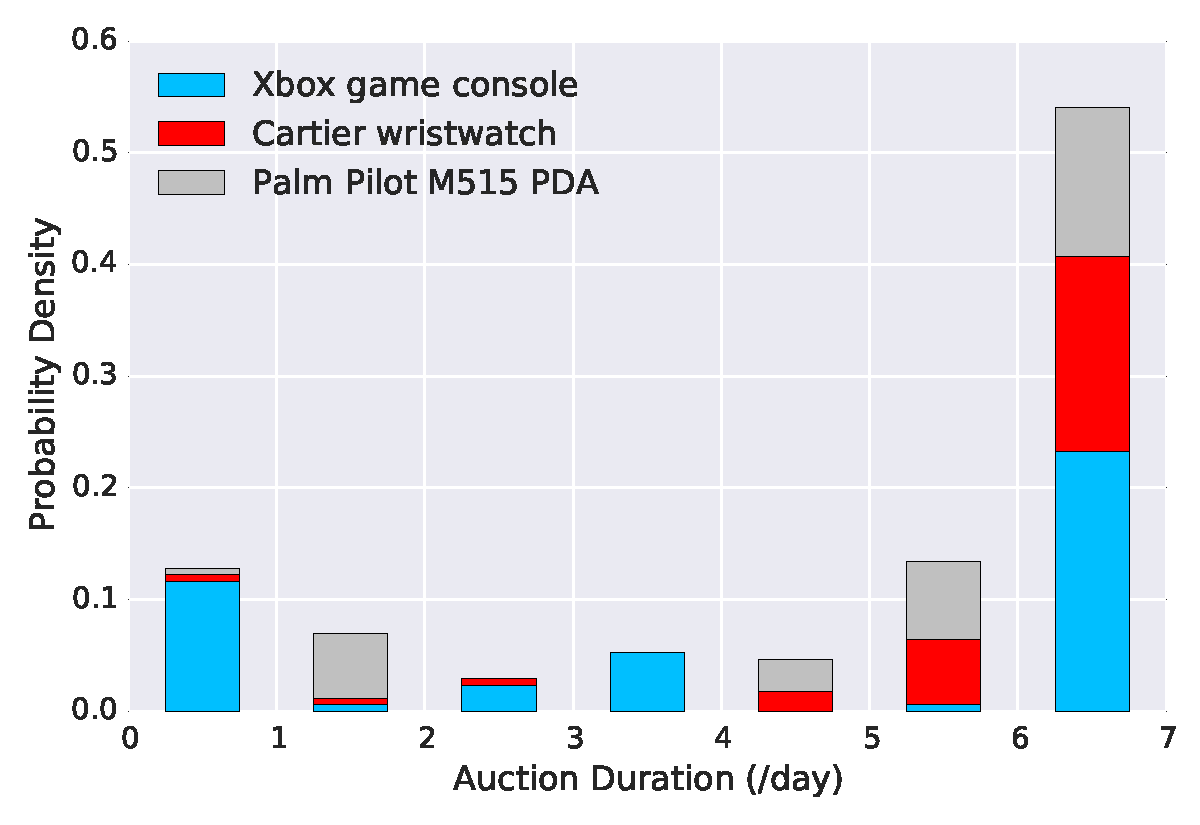
\includegraphics[width=0.55\textwidth]{chapter4/7_days_hist}}
   \bicaption[fig:number of bidders distribution histogram]{竞拍参与人数分布直方图}{竞拍参与人数分布直方图}{Fig}{Number of bidders distribution histogram}
 \end{figure}

目前,在在线拍卖市场上有两大类方法终止拍卖,分别是硬结束时间 (hard deadline) 和软结束时间 ("going, going, gone")。前一个,硬结束时间被eBay Live Auction采用:超过了硬结束时间的竞拍是不被接受的。后者,软结束时间被Amazon Auction使用\cite{amazonauction},在Amazon的在线拍卖市场上,拍卖持续时间会被自动延长只要在结束时间之前有新的竞拍。Roth和Ockenfels\cite{Roth2002Last}发现延迟竞拍 (late bidding) 和狙击竞拍 (snipe bidding) 时常发生在硬结束时间的在线拍卖中,比如eBay Live Auction。我们从eBay Live Auction收集到的真实买拍数据中也发现了这个现象。图\ref{fig:number of bidders distribution histogram}是在三种不同持续时长下的三种不同物品的在线拍卖。可以从这三幅子图中看出,竞拍者大多数会“挤”在拍卖的最后一天参与拍卖。Pinker\cite{Pinker2003Managing}称当在线拍卖网站流量很低的时候,延长拍卖在一定程度上可能有助于提高成交价。然后,这并不意味着可以一味地延长拍卖时间。Ariely等人\cite{Dan2003Buying}却认为即使更短的拍卖持续时间可能会只吸引更少的竞拍者,但是这样能增加竞拍者之间的竞争激烈度。他们在自己的实验中记录到拍卖时长是与成交价呈负相关关系。在本文中,为了更好地对在线拍卖竞拍者参与过程进行动态建模,我们将竞拍人数考虑成为拍卖持续时间的分段函数。

\subsection{起拍价与保留价}

起拍价可以理解成为另一种形式的保留价,通常是要么公开,要么保密。起拍价迫使竞拍者需要竞拍时高于起拍价。而保留价是拍卖者为成交价设定的一个下限。如果竞拍结束时,最高竞拍价还低于保留价的话,那么卖家有权利撤销这次拍卖。

从大量的拍卖记录中,我们发现如果竞拍者人数不够的话,那么最终成交价就会比较低。而竞拍者人数不仅仅与竞拍持续时间也与起拍价相关。Vakrat等人\cite{Pinker2001Using}经过分析实例发现当没有起拍价限制时,拍卖品会以低于相应零售商给出的价格很多的成交价被拍出。当起拍价增加时,成交价很大可能会趋近于起拍价。如果起拍价进一步增加,拍卖流拍的可能性会骤增。Reiley等人\cite{Ockenfels2006Online}发现设置了公开的起拍价和保留价后会减少竞拍人数,并且也会增加拍卖品流拍的可能性。同样地,Ariely等人\cite{Dan2003Buying}发现了起拍价和成交价之间具有正相关关系。即使一个很低的起拍价会吸引更多的竞拍者,但是竞拍者的出价会很低,不足以在拍卖者之间产生价格竞争。此外,通过大量的实例调查,Bradlow等人\cite{Bradlow2007Bayesian}发现起拍价与竞拍时间的增幅是具有负相关关系的。这也意味着一个低的起拍价会在短时间吸引更多的竞拍者。在本文提出的在线拍卖模型中,我们将起拍价就认为是保留价,以期望去探索发现保留价和卖家期望收益的关系。

\section{基于信息熵的在线拍卖模型}
在本小节中,我将陈述基于信息熵的在线拍卖模型。首先,用$\lambda_t$表示在线拍卖开始时间t后单位时间内的竞拍者到达率。值得指出的是,$\lambda_t$是与许多因素相关的,比如拍卖持续时间、当前参与拍卖人数、当前最高价以及竞拍规则。当然,肯定还有其他因素影响着在线拍卖。在真实情况中,在时间段$[t,t+\delta t]$内到达的竞拍者人数是一个随机变量。Vakrat和Seidmann\cite{Vakrat2000Implications}发现在线拍卖中新竞拍者的到达过程与指数分布非常相似。为了简化竞拍者的到达过程,同时也为了更好的抓住在线拍卖的动态特征,Chen等人\cite{Chen2007Optimal}将在线拍卖的竞拍者到达过程拟合成了一个泊松分布。该泊松分布的参数设为$\lambda$,可认为是在线拍卖中的竞拍者到达率。具体的,$N$个竞拍者在时间长度$t$内到达的概率质量函数被定义为:
\begin{equation}
\label{eq:number of bidder}
P_t(N=n)=\frac{e^{-\lambda t}(\lambda t)^n}{n!},n=0,1,2,...
\end{equation}

然而,在实际的在线拍卖中,到达率$\lambda$并不会全程保持不变。我们可以从图\ref{fig:number of bidders distribution histogram}发现到达率$\lambda_t$在在线拍卖过程中是变化的。为了比Chen等人提出的模型更好地抓住在线拍卖的动态特征,我们将拍卖持续时长$[0,T]$切分为一组不重叠的子区间,以使得到达率$\lambda_t$在不同子区间内取不同的值,然而在子区间内保持不变。

在我们的模型中,在线市场的数据卖家会列出他们要出售数据商品$D$的一些指标,去帮助买家估计该商品的价值。这些指标有$H(D)$,数据信息熵\cite{li2017first};$s(D)$,数据集的大小;或者是数据集的生成时间等等。每一个潜在竞拍者都会在参加拍卖前浏览这些信息。利用这些信息,潜在的拍卖者可以给待拍卖的商品估计出一个价值区间$[v_l,v_h]$。因为,本文主要关注基于信息熵的在线拍卖,我们将这一估计过程定义为如下:
\begin{equation}
\label{eq:v_l}
%v_l=\frac{H(x)}{s(x)},
v_l \propto H(D),
\end{equation}
\begin{equation}
\label{eq:v_h}
v_h \propto\alpha H(D),\alpha\ge 1,
%v_h=\alpha\frac{H(x)}{s(x)},\alpha\ge 1,
\end{equation}

其中,$\alpha$是放大系数。

在在线拍卖中,我们用元组$(a_i,b_i)$分别表示竞拍者$i$的到达时刻和出价。出价$b_i$是与拍品的真实价值$v_i \in [v_l,v_h]$相关的,记为$b_i=b(v_i)$。如果在时刻$t$有$n_t$个竞拍者参与当次拍卖,对于当前时刻$t$,我们将这些竞拍者记为一个集合$B$。在这个集合中,对于所有的竞拍者,其到达时间$a_i \le t, i=1,2,...,n_t$。这些竞拍者的出价构成一个出价向量$\vec{b}_t=(b_1,b_2,...,b_{n_t})$。

现在我们已经为时刻$t$的在线拍卖定义了两个状态变量$n_t$和$\vec{b}_t$。如果此次拍卖中有$k$个物品要拍卖。那么在拍卖的结尾时,那么将会有一个成交价向量$\vec{p}=(p_1,p_2,...,p_k)$。这个成交价向量是竞拍总人数$n_T$,竞拍出价向量$\vec{b}_T$,状态变量的最终值以及拍卖规则$\textbf{R}$的函数。对于卖家而言,他的目标是最大化拍卖物品的成交价,即:

\begin{equation}
\max_{\textbf{R},T} \arrowvert \vec{p}(n_T,\vec{b}_T) \arrowvert_1,
\end{equation}

其中$\arrowvert\cdot\arrowvert_1$是向量的$L_1$范数。拍卖规则$\textbf{R}$规定着1)拍卖结束时商品是如何分配的;2)成交价是如何决定的;3)出价是公开还是密封的;4)是否有保留价;5)保留价是公开的还是密封的等等\cite{Pinker2003Managing}.。假设卖家为每一个竞拍者设计一个估价区间$V_i=[v_l,v_h]$。令$V=\prod_{i=1}^{n}V_i$,表示所有竞拍者联合估价。除此以外卖家还需要设计分配规则$q(v)$对于每一个联合估价$v \in V$。具体来说,$q(v)=(q_1(v),q_2(v),...,q_n(v))$是一个概率向量,其中$q_i(v)$是第$i$个竞拍者赢得拍品的概率。此外,本文还定义了一个支付向量$p(v)=(p_1(v),p_2(v),...,p_n(v))$,其中$p_i(v)\in \mathbb{R}$是第$i$个竞拍者期望支付价格。因为参加拍卖是自愿的,我们假设对于每个竞拍者$i$,如果他的估价低于卖家的最低价,那么他会选择不参加此次竞拍,即$np \in V_i$。具体来说,如果$v\in V$并且$v_i=np$, 那么 $p_i(v)=0$且$q_i(v)=0$。

现如今,英式拍卖,荷兰式拍卖,第一价格拍卖以及第二价格拍卖是最普遍也是被研究地最多的四种拍卖机制。尤其是英式拍卖如今最流行的。在开始陈述本文提出的模型之前,需要作出以下假设:

\begin{assmp}[个人估价私密性]
\label{conj:private value}
  对于竞拍者$i$,他对拍卖品的估价$v_i$是只有他自己知道的,卖家和其他竞拍者是不清楚的。但是所有拍卖参与者都默认$v_i$是一个落在区间$[v_l,v_h]$的随机变量,还知道其概率分布函数$F_i(v_i)=\int_{v_l}^{v_i}f_i(z)dz$,其中$f_i$是严格大于零的连续密度函数。
 
\end{assmp}

\begin{assmp}[估价的独立性]
\label{conj:independent value}
  简单来说,每个竞拍者的估价$v_1,v_2,...,v_n$是独立的,也就是说$v_1,v_2,...,v_n$的联合概率分布函数为
  \begin{equation}
	F(v_1,v_2,...,v_n)=F_1(v_1)F_2(v_2)...F_n(v_n).
	\end{equation}
 
\end{assmp}

\begin{assmp}[估价分布函数的对称性]
\label{conj:symmetric distribution function}
这些概率分布函数是相同的,对于所有的$i,j=1,2,...,n$ 和 $v\in[v_l,v_h]$,有
	\begin{equation}
	F_i(v)=F_j(v)=F(v).
	\end{equation}
 
\end{assmp}

\begin{assmp}[竞拍者风险中立]
\label{conj:risk nuetral}
对于每个竞拍者,他的目标是最大化其期望收益。
 
\end{assmp}

\begin{assmp}[无串通性]
\label{conj:no collusion}
每一个竞拍者都是独立地决定其竞拍策略,在竞拍者之间没有串通。
\end{assmp}

不同于传统拍卖,在线拍卖并不需要召集所有的参与者到拍卖行中。因此,在线拍卖的竞拍者之间串通的可能性是远远小于传统拍卖的。

以上所有假设描述了对称独立私有价值条件(Symmeteric Independent Private Value, SIPV)。对于卖家来说,Meyerson\cite{Myerson1981Optimal}发现了在前面提到过的四种拍卖机制下收益是等价的。由于收益等价定理,在某种程度上来说,以上四种拍卖机制是等价的。本文选择在对称独立私有价值条件下的第二价格拍卖作为在线拍卖机制。为不失一般性,本文将第二价格拍卖扩招到适用于$k$物品的第$k$价格拍卖。本文形式化地将对于数据商品的在线第$k$价格拍卖描述在算法xx中。



\subsection{带保留价的单件物品在线拍卖}

在本小节中,我们先讨论设置了公开保留价的单件商品的在线拍卖,也就是这里的$k=1$。在传统的第二价格拍卖中,Riley和Samuelson\cite{Riley1981Optimal}得出了这样的结论:当对称独立私有价值条件满足时,对于设置了合适的保留价$r$和有$n$个竞拍者的在线拍卖,卖家的期望收益为:
\begin{equation}
\label{eq:basic expected revenue}
R_s=n\int_{r}^{v_h}(xf(x)+F(x)-1)F^{(n-1)}(x)dx.
\end{equation}

在单件商品在线拍卖中,数据卖家只卖出一件数据商品。因为在在线拍卖中,竞拍者人数$N$也是一个随机变量,卖家的期望收益应当是与$N$有关的,即:

\begin{equation}
\label{eq:basic online expected revenue}
R_s^{online}=E_N(R_s).
\end{equation}

Chen等人\cite{Chen2007Optimal}将竞拍者参与在线拍卖的过程建模为一个到达率为常量$\lambda$的泊松过程。本文提出的在线拍卖模型也是一个泊松过程,但是该到达率



\subsection{带保留价的多件物品在线拍卖}

\section{模型评估}

\section{本章小结}